% !TEX root = ../thesis.tex
%
\chapter{Einleitung}
\label{sec:intro}
Wikipedia ist die bekannteste freie Wissenssammlung im Internet.
Bei fast 50 Millionen Artikeln in 278 Sprachen\footnote{https://stats.wikimedia.org/DE/TablesArticlesTotal.htm} Anfang 2019 sind Informationen zu einer Vielfalt an Themen verfügbar.
Sogar YouTube und Facebook greifen auf Wikipedia zurück, um zusätzliche Informationen zu kontroversen Themen zu präsentieren.\cite{youtube-facebook-wp}

% Die große Menge an Information bietet allerdings auch Herausforderungen.
% Neben dem reinen Zusammenstellen ist auch der einfache Zugang zu den Informationen wichtig.

Die Darstellung der Informationen in natürlicher Sprache als Textartikel ist für Menschen praktisch.
Doch für maschinelle Verarbeitung ist diese unstrukturierte Form der Darstellung nicht so gut geeignet, zumal sich die Fakten je nach Sprachversion auch unterscheiden können.
Um diesem Problem zu entgegnen wurde 2012 das Wikidata Projekt gegründet, mit dem Ziel, die Informationen aus Wikipedia in atomare Aussagen zerlegt strukturiert zu verwalten\cite{wikidata}.
Genau wie Wikipedia selbst kann auch Wikidata ohne Beschränkungen frei bearbeitet werden.

Ein Beispiel für die Datenrepräsentation in Wikidata zeigt \cref{fig:sample-statement}.
Mit Wikidata ist es möglich, auch verschiedene zunächst widersprüchlich erscheinende Fakten parallel darzustellen.
Abhängig von der Art der Bestimmung (\emph{determination method}) können entweder der Mount Everest oder auch Chimborazo als höchster Punkt der Erde gesehen werden.
Diese Flexibilität ist notwendig, weil Wikidata ein Community-Projekt ist und deswegen auch die Möglichkeit haben muss, Fakten differenziert abzubilden um Konsens zu erreichen.
Wie man im Beispiel sieht, können Statements zusätzlich auch noch mit Referenzen untermauert werden.
Um Mehrdeutigkeiten zu vermeiden, werden alle Entitäten in Wikidata durch eindeutige IDs referenziert, und Statements verlinken auf diese IDs.

Für viele Projekte sind die Daten aus Wikidata aufgrund dieser Eigenschaften besonders interessant.
So können die IDs zur eindeutigen Unterscheidung verschiedener Konzepte dienen und gleichzeitig noch weitere mit diesen Konzepten verlinkte Informationen abgerufen werden.
Auch die Mehrsprachigkeit der Daten ist zur Zuordnung von gleichen Konzepten unterschiedlicher Sprachen sehr nützlich.
Der kollaborative Aspekt von Wikidata wirft weitere interessante Fragestellungen, zum Beispiel zur Qualität der Daten\cite{wd-taxonomic-hierarchies} oder der Verwendung von Referenzen\cite{wd-wk-common-references}\cite{wd-provenance-information}.

Wikidata bietet bereits mehrere Wege für den Zugang zu den Daten an.
Für einfache Abfragen zu einzelnen Objekten gibt es die Wikidata API, für komplexere Abfragen die auch Relationen zwischen mehreren Entitäten nutzen bietet sich der Wikidata Query Service an. 
Außerdem werden Datenexports sowohl in einem Wikidata eigenen JSON-basierten Format sowie als RDF angeboten.

Doch durch das Wachstum von Wikidata sind neue Methoden zum Zugang zu den Daten notwendig.
Mittlerweile besteht Wikidata aus mehr als 700 Million Statements zu fast 60 Millionen Items.
Die vollständigen RDF-Datenexporte sind damit selbst komprimiert über 50 GB groß, und der Wikidata Query Service produziert Timeouts nicht aufgrund der Komplexität der Anfrage, sondern weil zu viele Daten abgefragt werden.\cite{wd-wk-common-references}.
Es fehlt also ein System für den Bereich zwischen Abfragen kleinerer Datenmengen (Wikidata API, Wikidata Query Service) und dem Verarbeiten vollständiger Exporte.
Als Lösung für dieses Problem wird in dieser Arbeit ein System vorgestellt, welches nach Angabe von Filterkriterien Dumps mit einer Teilmenge der Daten generieren kann. 

\begin{figure}
  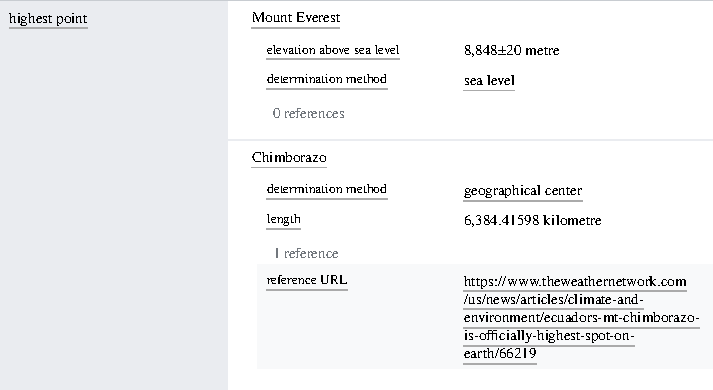
\includegraphics[width=\linewidth]{pics/example-statement}
  \caption{Zwei Statements des Items ``Erde'' für die Property ``höchster Punkt''}
  \label{fig:sample-statement}
\end{figure} 

\section{Struktur der Arbeit}
Im zweiten Kapitel wird zunächst notwendiges Hintergrundwissen zum Aufbau von Wikidata und den verwendeten Technologien vermittelt.
Danach werden in \cref{chap:requirements} die Anforderung an das System detaillierter beschrieben und verwandete Arbeiten verglichen.
In \cref{chap:design} wird dann das Design der System erarbeitet, dessen Implementierung in \cref{chap:implementation} vorgestellt wird.
In der folgenden Evaluation in \cref{chap:evaluation} wird die Implementierung auf Erreichen der Anforderung geprüft und auch ein Vergleich mit den existierenden Wikidata-Dumps vorgenommen.
Im letzten Kapitel \cref{chap:conclusion} wird schließlich auf mögliche zukünftige Verbesserungen eingegangen, bevor ein Fazit gefällt wird.

Dabei werden die folgenden Beiträge geleistet:
\begin{itemize}
  \item Analyse verschiedener Systemdesigns zur Generierung angepasster Wikidata-Dumps
  \item Entwurf einer Spezifikation für Filterkriterien
  \item Implementierung des vorgestellten Designs mit Wikidata-Toolkit
  \item Evaluation der Vollständigkeit und Korrektheit des RDF-Exports in Wikidata-Toolkit
\end{itemize}